\subsection{the Continuum Drug Spread Model}
Our model is inspired by the Porous Media Contaminant Transport Model.\cite{8} The transport process is expressed in a differential equation, balancing the total mass of contaminant in the fracture. 

Similarly, we propose a Continnum Drug Spread(CDS) model. This model, which is expressed in a \textbf{\itshape partial differential equation}, is constructed under the assumption that we view the geographical features in a continuous way. 

Let $S(x,y,t)$ represent the amount of drug stored in $(x,y)$ at time $t$. The NFLIS data contains drug identification counts in years 2010-2017 for narcotic analgesics and heroin in each of the counties from the five states stated in the \textit{problem background} section, which we denote as $F(x,y,t)$, the amount of drugs identified in $(x,y)$ at time $t$. We assume that the amount of identified drugs is directly proportional to the total amount of drugs with a proportionality constant $k$, such that
\begin{equation}
S(x,y,t) = k\cdot F(x,y,t)
\end{equation}

We denote the total amount of drug used in $(x,y)$ at time $t$ with $U(x,y,t)$, and since the amount of drug used is less or equal to the amount of drug stored in the same location at the same time, we have
\begin{equation}
U(x,y,t) = \lambda S(x,y,t), 0\leq \lambda \leq 1
\end{equation}

It is natural to assume that $\lambda$ is revelant with socio-economical factors of the given location. We shall address this in the second part of the problem.

Intuitively, $D(\frac{\partial^2 S}{\partial x^2} + \frac{\partial^2 S}{\partial y^2})$ can be used to describe the total amount of drug transported into the city. $\frac{\partial^2 S}{\partial x^2} + \frac{\partial^2 S}{\partial y^2}$ describes the \textit{emergency} of transporting drugs, i.e. the trend of transporting drug from $(x,y)$ to neighboring coordinates.

The difference between the total amount of drug transported into $(x,y)$ and the amount of drug used equals to the change of storage:

\begin{equation}
D(\frac{\partial^2 S}{\partial x^2} + \frac{\partial^2 S}{\partial y^2}) - \lambda S = \frac{\partial S}{\partial t} 
\end{equation}

$S$, however, is unknown. We substitute (1) into (3), and eliminate the common factor $k$ from both sides of the equation
\begin{equation}
D(\frac{\partial^2 F}{\partial x^2} + \frac{\partial^2 F}{\partial y^2}) - \lambda F = \frac{\partial F}{\partial t}
\end{equation}

\subsection{Analytical Solution to the CDS Model}

\subsection{Identify the Origin of Specific Opioid Use}
We compose a 3D image describing the characteristics of the reported synthetic opioid and heroin cases across counties. We transform the FIPS coding of the counties into their latitude and longitude. The x-axis represents the latitude, the y-axis represents the longitude, and the z-axis represents the specific drug reports.

We comopose a continuous 3D model of the latitude-longitude-drugreport relationship using quadratic interpolation. According to our assumption(A1-2), a Producer of a specific opioid use should reach a local maxima in drug reports. An Origin, which is a subset of Producers, possess the same statistical feature. A contour map(Figure 1(a)) is composed to visualize this ideology.

\begin{figure}[H]
	\centering
	\subfigure[3D Plot]{
		\centering
		\begin{minipage}[t]{0.3\linewidth}
			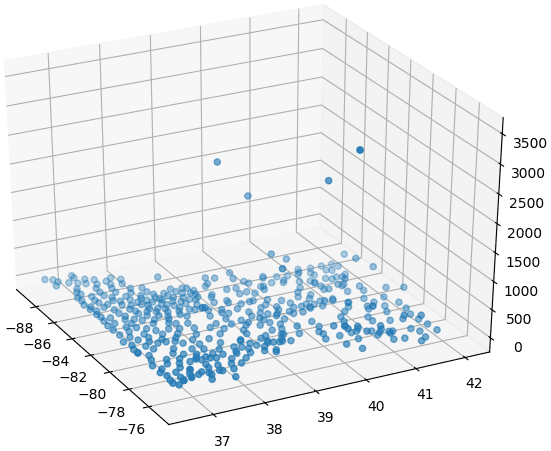
\includegraphics[width=2in]{001}
		\end{minipage}
	}
	\subfigure[Contour Map]{
		\centering
		\begin{minipage}[t]{0.4\linewidth}
			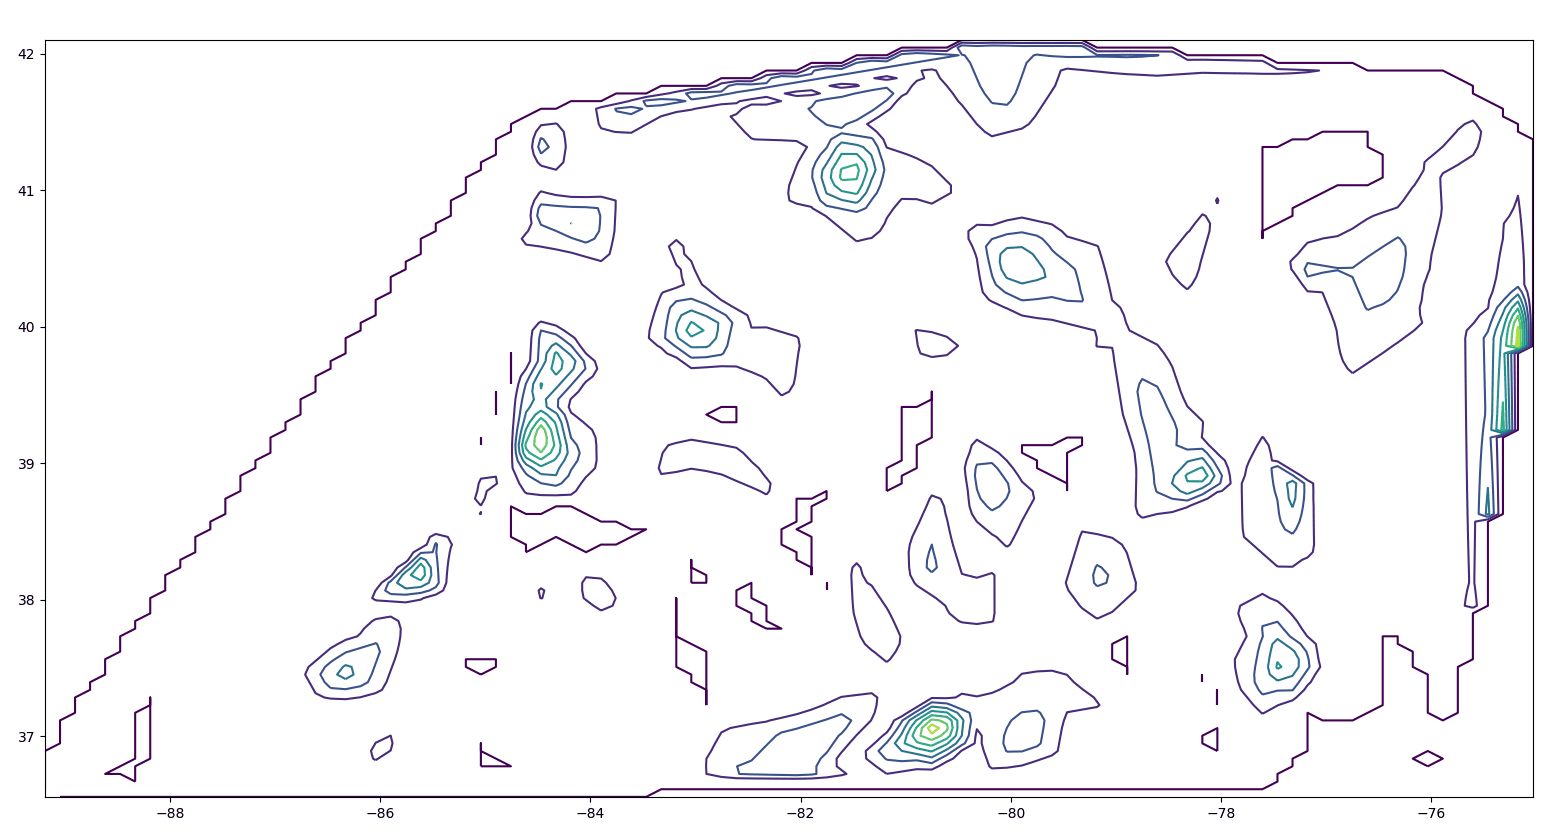
\includegraphics[width=3in]{000}
		\end{minipage}
	}
	\caption{Heroin}
\end{figure}

As illustrated in A3, not all Producers are Origins. Therefore, not all local maximum indicate Origins. We need to set up a threshold to distinguish Producers from Origins. 

Therefore, we identify the possible locations where specific opioid use might have started by computing all local maxima(see algorithm 1), and rank them to find the possible origins in each of the five states. The details of our ranking scheme concerns a comparison of a certain county's data in time. If a county remains a Producer(i.e. local maxima) for six years in a row, then we define it as a \textbf{\itshape Potential Origin}. For each state, if the number of Potential Origins is greater than 3, then we select three Potential Origins with top three specific opioid reports as the possible Origins for the opioid in discussion of that state.



\subsection{Drug Identification Threshold}
We endeavor to propose a drug identification threshold such that when a county's total opioid report reaches this threshold, the U.S. government should be extremely concerned with opioid control in this county.

Statistics from the dataset reveal that on average, 92 cases of opioid identifications occur in a county per year. Traversing the map, we find that in counties with severe drug crisis, thousands of opioid identification may occur per year. Under this premesis, we classify the Producers into three levels(see Table 2).

\begin{table}[H]
	\centering
	\begin{tabular}{|c|c|}
		\hline
		\rowcolor[HTML]{656565} 
		{\color[HTML]{FFFFFF} \textbf{Level}} & {\color[HTML]{FFFFFF} \textbf{Threshold}} \\ \hline
		First-Level Origin  & total Drug Report per year $\geq 1000$ \\ \hline
		Second-Level Origin & $100 \leq$ total Drug Report per year $\leq 1000$ \\ \hline
		Third-Level Origin  & total Drug Report per year $\leq 100$ \\ \hline
	\end{tabular}
	\caption{Notations}
\end{table}

These three levels indicate the degree at which the U.S. government need to be alarmed. First level origins are counties with severe opioid crisis. Third-level origins are those with minor opioid crisis. The second level is in-between.

The strategy against different level of origins vary. First level origins require immediate control and intervention, while third level origins could be treated with a mild approach. For origins in the second level, the government need to focus specifically on those in danger of transforming from the second to the first level.

\subsection{Model Prediction via the Grey Method}
The database provides us with the record of total drug identification cases from 2010 to 2017. We could use Grey Method to predict the future data based on our current model.

The Gray Model is applied mainly on incomplete data and undeterminable problems. We the use GM(1,1) model for prediction.\cite{13}

Let $X$ be a sequence of observed data, such that
\begin{equation}
X^{(0)} = (X^{(0)}(1),X^{(0)}(2),\cdots,X^{(0)}(n))
\end{equation}
Here, $X^{(0)}(i)$ represents the observed data at time $i$. We generate the first-order Accumulated Generating Operation sequence  $X^{(1)}(i)$ based on $X^{(0)}(i)$, where
\begin{equation}
X^{(1)}(i) = \sum_{k=1}^i X^{(0)}(k) = X^{(1)}(i-1)+X^{(0)}(i)
\end{equation}
Then we establish the first-order differential equation of $X^{(1)}(i)$ as
\begin{equation}
\frac{dX^{(1)}}{dt}+aX^{(1)}=u
\end{equation}
where $a$ and $u$ are parameters we wish to obtain. (6) and (7) reveal that
\begin{equation}
\hat{X}^{(1)}(i+1) = (X^{(0)}(1)-\frac{u}{a})e^{-ai}+\frac{u}{a}
\end{equation}
Now we attempt to fit parameter $a$ and $u$, as described in (7). Let $\hat{a}$ be a sequence of parameters where $\hat{a}=[a,u]^T$. The solution to $\hat{a}$ is
\begin{equation}
\hat{a} = (B^T B)^{-1}B^TY_n
\end{equation}
where
\begin{equation}
B=\left[
\begin{array}{cc}
-\frac{1}{2}[X^{(1)}(1)+X^{(1)}(2)] & 1\\
-\frac{1}{2}[X^{(1)}(2)+X^{(1)}(2)] & 1\\
\cdots & \cdots \\
-\frac{1}{2}[X^{(1)}(n-1)+X^{(1)}(n)] & 1\\
\end{array}
\right],
Y_n = [X^{(0)}(2),X^{(0)}(3),\cdots, X^{(0)}(n)]^T
\end{equation}






